\part{More complex meshes}
\frame{\partpage}

\begin{frame}{Winding order}
	\begin{itemize}
		\pause\item It is sometimes important to know which side of a triangle is the ``front'' and which is the ``back''
		\pause\item OpenGL determines this by \textbf{winding order}
	\end{itemize}
	\begin{columns}
		\pause
		\begin{column}{0.48\textwidth}
			\begin{center}
				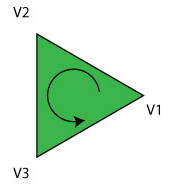
\includegraphics[width=0.5\textwidth]{winding_ccw}
				
				If the vertices go \textbf{anticlockwise}, you are looking at the \textbf{front}
			\end{center}
		\end{column}
		\pause
		\begin{column}{0.48\textwidth}
			\begin{center}
				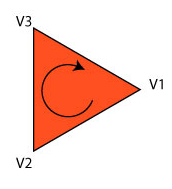
\includegraphics[width=0.5\textwidth]{winding_cw}
				
				If the vertices go \textbf{clockwise}, you are looking at the \textbf{back}
			\end{center}
		\end{column}
	\end{columns}
\end{frame}

\begin{frame}[fragile]{Backface culling}
	\pause
	\begin{lstlisting}
glEnable(GL_CULL_FACE);
	\end{lstlisting}
	\begin{itemize}
		\pause\item This will cause only the front faces of triangles to be drawn
		\pause\item Triangles whose front face is not visible will be \textbf{culled}
		\pause\item Culled faces are not passed through the rasteriser or fragment shader
		\pause\item Saves time, and should make no difference to appearance ---
			as long as all meshes are closed and have correct winding
	\end{itemize}
\end{frame}

\begin{frame}[fragile]{When backface culling goes bad?}
	\begin{center}
		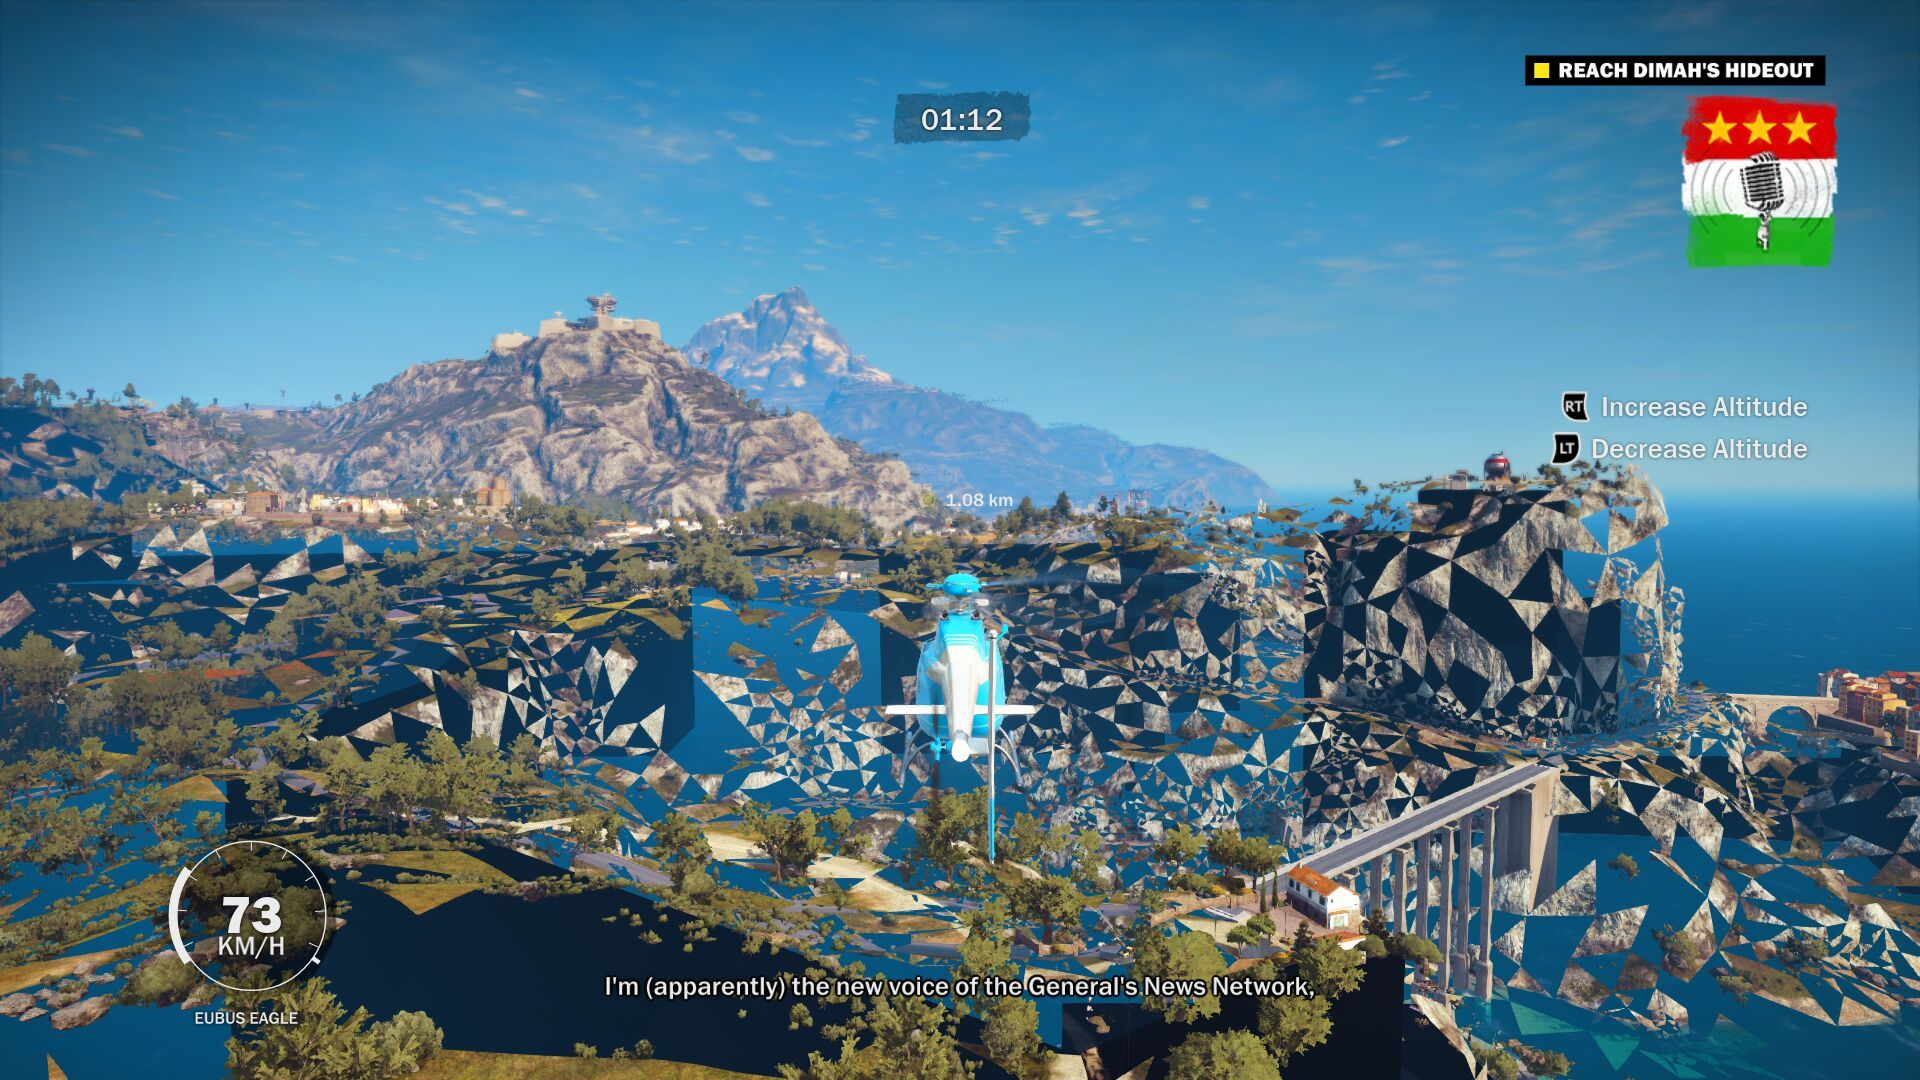
\includegraphics[width=\textwidth]{missing_triangles}
	\end{center}
\end{frame}

\begin{frame}{Let's draw a square!}
	\begin{center}
		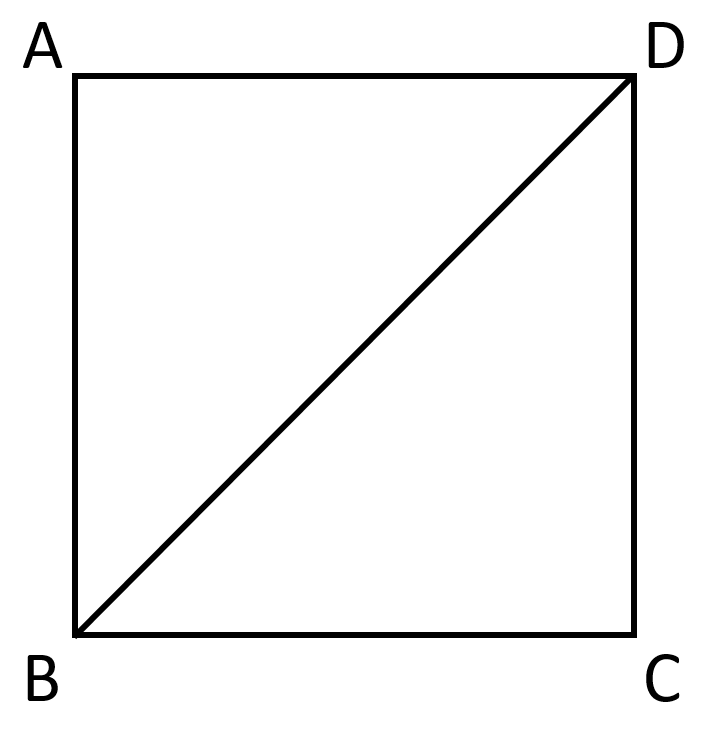
\includegraphics[height=0.8\textheight]{square_vertices}
	\end{center}
\end{frame}

\begin{frame}{Let's draw a cube!}
	\begin{center}
		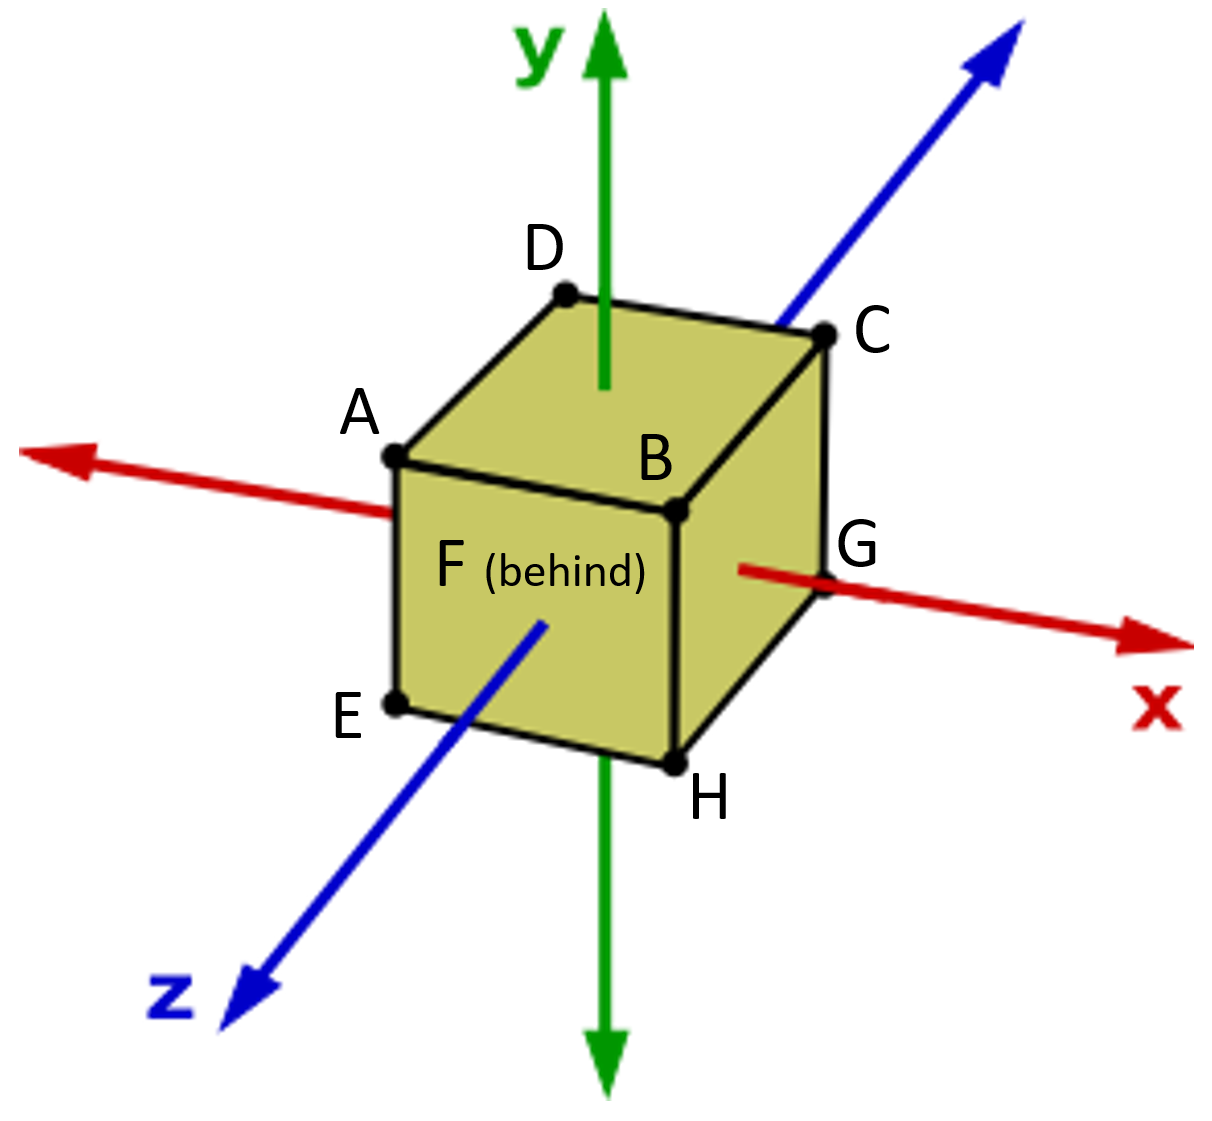
\includegraphics[height=0.8\textheight]{cube_vertices}
	\end{center}
\end{frame}

